% Created 2017-12-12 Tue 16:18
% Intended LaTeX compiler: pdflatex
\documentclass[11pt]{article}
\usepackage[utf8]{inputenc}
\usepackage{lmodern}
\usepackage[T1]{fontenc}
\usepackage{fixltx2e}
\usepackage{graphicx}
\usepackage{longtable}
\usepackage{float}
\usepackage{wrapfig}
\usepackage{rotating}
\usepackage[normalem]{ulem}
\usepackage{amsmath}
\usepackage{textcomp}
\usepackage{marvosym}
\usepackage{wasysym}
\usepackage{amssymb}
\usepackage{amsmath}
\usepackage[version=3]{mhchem}
\usepackage[numbers,super,sort&compress]{natbib}
\usepackage{natmove}
\usepackage{url}
\usepackage{minted}
\usepackage{underscore}
\usepackage[linktocpage,pdfstartview=FitH,colorlinks,
linkcolor=blue,anchorcolor=blue,
citecolor=blue,filecolor=blue,menucolor=blue,urlcolor=blue]{hyperref}
\usepackage{attachfile}
\author{Jan}
\date{\today}
\title{Open source}
\begin{document}

\setcounter{tocdepth}{1}
\tableofcontents


\section*{Introduction}
\label{sec:org53c900f}

\begin{itemize}
\item Illustration of why open source can be useful to academics
\item the open source tool that I use most often is emacs
\end{itemize}

\section*{Why I love emacs}
\label{sec:orga8467e8}
\subsection*{what is emacs?}
\label{sec:org826b2b5}
\begin{itemize}
\item an editor which was designed in the 70s
\item it is open source so the whole world can contribute
\item unlike MS Word, the people "working on" emacs are "like us"
\item I use "org-mode" developed by \href{https://staff.fnwi.uva.nl/c.dominik/}{Carsten Dominik} at UvA
\item with customizations by \href{http://kitchingroup.cheme.cmu.edu/scimax}{John Kitchin} at Carnegie Mellon
\end{itemize}

\subsection*{emacs contributers}
\label{sec:org490b9dc}
\begin{itemize}
\item type papers in latex
\item bibliographies in bibtex: C-c ]
\item work with data
\item program
\item have admin tasks: someone walks in and you have to remember something: C-M-r
\item teach students: \url{https://github.com/jkitchin/techela}
\end{itemize}


\subsection*{why is it great?}
\label{sec:org12e3006}
\subsubsection*{amazing editor}
\label{sec:org74aa4cf}
\begin{itemize}
\item edit columns: get rid of the 2's
\end{itemize}

111333222
111333222
111333222
111333222

\begin{itemize}
\item change structure of file
\end{itemize}
\subsubsection*{latex stuff}
\label{sec:org837b86d}
\begin{itemize}
\item equations
\label{sec:org5651b1a}
\begin{itemize}
\item this is an org-file but the latex things work in latex as well
\item use M-x org-cdlatex-mode
\item add equation
\end{itemize}

\begin{equation}
\label{eq:2}
ref:eq:5
\end{equation}

here are some other equations

\begin{equation}
\label{eq:4}
\frac{1}{3} = x^2
\end{equation}

\begin{equation}
\label{eq:5}
ax^2+bx+c=0
\end{equation}

\begin{equation}
\label{eq:6}
ax^2+bx+c=0
\end{equation}

\item refer to equations and export to latex
\label{sec:org9af59bb}
\begin{itemize}
\item refer to an equation with C-c (
\item export to latex: C-c C-e
\item but you can also export to html and reveal
\item export with ox-manuscript: generates submission letter as well

\item easy to add links e.g. to a \href{econometrics.org}{presentation at slide Data science}
\item or to a \href{bibtexfile.bib}{bib tex file}
\item add bibitex entry from doi-identifier: 10.1002/jae.896
\end{itemize}
\end{itemize}
\subsubsection*{highlighting}
\label{sec:org940a133}

\begin{itemize}
\item most latex editors do not allow for meta data in latex:
\item so most people make comments in bold in latex and pdf; then they send it to a conference\ldots{}
\item Use M-x ov-highlighter/body
\item So here we have some text.
\item and here we add some comments that will not be exported to pdf
\end{itemize}

\subsubsection*{tables}
\label{sec:org6f1774d}

\begin{itemize}
\item Latex is great, but not with tables\ldots{}
\item simple to add a table in emacs
\end{itemize}

\begin{center}
\begin{tabular}{lll}
1 & 2 & 3\\
\hline
a & a & a\\
b & b & b\\
 &  & \\
\end{tabular}
\end{center}

\begin{itemize}
\item you can do excel stuff with it: C-c \} to see "addresses"
\end{itemize}

\begin{center}
\label{data}
\begin{tabular}{rrrr}
col 1 & col 2 & col 3 & mean\\
\hline
6 & 5 & 10 & 7\\
6 & 8 & 9 & 7.6666667\\
4 & 4 & 5 & 4.3333333\\
\end{tabular}
\end{center}


\begin{minted}[frame=lines,fontsize=\scriptsize,linenos]{ipython}
import pandas as pd
import matplotlib.pyplot as plt

df = pd.DataFrame(dataset)
plt.scatter(df[0],df[1])
plt.savefig('table.png')
\end{minted}



\begin{center}
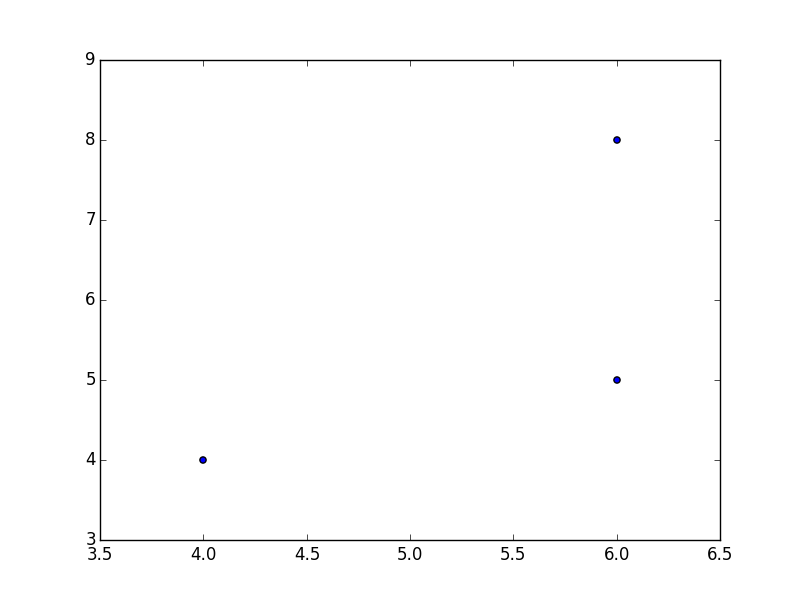
\includegraphics[width=.9\linewidth]{./table.png}
\end{center}

\subsection*{To do lists}
\label{sec:org7c5a1fa}

\subsubsection*{{\bfseries\sffamily TODO} bla bla bla; use C-c C-t}
\label{sec:org044fe3e}

\begin{itemize}
\item to add a date: C-c C-s
\end{itemize}

\subsection*{great extensions}
\label{sec:org2b769ec}
\begin{itemize}
\item emacs spotify mode
\item emacs weather mode
\item emacs git: magit
\end{itemize}
\section*{Conclusion}
\label{sec:orgdc8da81}

\begin{itemize}
\item point is not that you have to use emacs
\item but when you come across something in open source, you should certainly try it!
\end{itemize}
\end{document}